\documentclass[11pt,t]{beamer}
\usetheme{metropolis}
\metroset{progressbar=frametitle,numbering=fraction}
\usefonttheme[onlymath]{serif} % serif math: proper primes, hats and italics
\usepackage{bm}
\usepackage{amsmath,amssymb,amsfonts}
\usepackage{mathrsfs}
\usepackage{booktabs}
\usepackage{graphicx}
\usepackage{xcolor}
\usepackage{tikz}
\usetikzlibrary{calc,positioning,decorations.pathmorphing}
\setbeamercolor{block title}{use=normal text, fg=normal text.fg,bg=normal text.bg!80!fg}
\setbeamercolor{mymath}{use={block title, normal text}, bg=block title.bg!50!normal text.bg}
\setbeamercolor{mymath2}{bg=blue!10, fg=black}
\graphicspath{{./figures/}{./logo/}{../PINN_for_FRG/figure/}}

%%%%%%%%%%%%% Macros %%%%%%%%%%%%%
\newcommand{\rmi}{\mathrm{i}}
\newcommand{\rmd}{\mathrm{d}}
\newcommand{\blockbodygap}{\vspace{0.3em}}
\newcommand{\afterblockgap}{\vspace{0.45em}}
\newcommand{\LN}{\mathrm{LN}}
\newcommand{\MeV}{\,\mathrm{MeV}}
\newcommand{\GeV}{\,\mathrm{GeV}}

\title{Solving Functional\\ Renormalization Group Equations\\ with Neural Networks}
\subtitle{}

\date{September 4, 2026}
\author{Yang-yang Tan}
\titlegraphic{%
  \begin{tikzpicture}[remember picture, overlay]
    % Top-left: conference name
    \node[anchor=north west, inner sep=0pt, font=\normalsize\bfseries, text=burgundy]
      at ([xshift=0.6cm,yshift=-0.5cm]current page.north west)
      {ERG2026, University of Sussex};
    % Bottom-right: UTokyo + IPI (aligned with author/date)
    \node[anchor=south east, inner sep=0pt] (utokyo) at ([xshift=-0.6cm,yshift=2.9cm]current page.south east) {%
      \raisebox{-0.5\height}{\includegraphics[height=3em]{UTokyo_Logotype_A_Color_RGB20240401.png}}%
      \hspace{0.4em}\rule[-0.9em]{0.4pt}{2em}\hspace{0.4em}%
      \raisebox{-0.5\height}{\includegraphics[height=2.3em]{ipilogo.png}}%
    };
    % Below UTokyo/IPI: RIKEN + iTHEMS (no separator)
    \node[anchor=north east, inner sep=0pt] at ([yshift=-0.5em]utokyo.south east) {%
      \raisebox{-0.5\height}{\includegraphics[height=2em]{logo_riken.pdf}}%
      \hspace{0.6em}%
      \raisebox{-0.5\height}{\includegraphics[height=2em]{logo_dark.pdf}}%
    };
  \end{tikzpicture}%
}

\definecolor{burgundy}{RGB}{127, 0, 32}
\definecolor{Kleinblue}{RGB}{0, 47, 167}
\newcommand{\running}[1]{\textcolor{burgundy}{#1}}
\newcommand{\kb}[1]{{\bfseries\color{Kleinblue} #1}}
% compact reference line at the bottom of a frame
% references pinned to the bottom of the page, independent of the frame content
\makeatletter
\newcommand{\refs}[1]{%
  \begin{tikzpicture}[remember picture, overlay]
    \node[anchor=south west, inner sep=0pt, align=flush left,
          text width=\dimexpr\textwidth-1.4cm\relax]
      at ([xshift=\beamer@leftmargin, yshift=0.6cm]current page.south west)
      {\raggedright\tiny\color{black!65} #1\par};
  \end{tikzpicture}}
\makeatother
\newcommand{\rtag}[1]{\textcolor{burgundy}{\textbf{#1}}}

\tikzset{
  stage/.style={
    rectangle, rounded corners=3pt,
    draw=#1!80, fill=#1!12, line width=0.8pt,
    minimum width=2.8cm, minimum height=1.7cm,
    align=center, font=\small\bfseries, text=#1!50!black,
    inner sep=4pt
  },
  tlarrow/.style={
    ->, >=stealth, line width=1.4pt, draw=gray!55,
    shorten >=2pt, shorten <=2pt
  }
}

\begin{document}
\begin{frame}[plain,noframenumbering,t]
  \inserttitlegraphic\par
  \vspace*{0.5cm}
  {\LARGE\bfseries \inserttitle\par}
  \vspace{0.5em}
  {\small\color{black!65} Phys.\ Rev.\ D \textbf{114}, 036026 (2026)\par}
  \vspace{0.4em}
  {\color{orange}\rule{\textwidth}{0.4pt}\par}
  \vspace{1.4em}
  {\normalsize\bfseries \insertauthor\par}
  \vspace{0.6em}
  {\small IPI, The University of Tokyo\par}
  \vspace{0.4em}
  {\small with \textbf{Wei-jie Fu}, \textbf{Lianyi He} and \textbf{Lingxiao Wang}\par}
  \vspace{0.3em}
  {\normalsize \insertdate\par}
\end{frame}

% ---------------------------------------------------------------- 0
\begin{frame}{Introduction}
  \begin{columns}[T,onlytextwidth]
    \begin{column}{0.54\textwidth}
      \small
      \kb{Wetterich equation}\\[0.1em]
      {\centering
        $\partial_t\Gamma_k=\tfrac12\,\mathrm{Tr}\!\left[\partial_t R_k\left(\Gamma_k^{(2)}+R_k\right)^{-1}\right]$\par}
      \vspace{0.2em}

      \kb{LPA}\quad flow of $V_k(\rho)$, a stiff PDE\\
      Taylor, grids, Chebyshev, DG/FEM, FV

      \vspace{0.3em}
      \kb{Bottleneck}\\
      stiffness, curse of dimensionality

      \vspace{0.2em}
      \uncover<2->{%
      \kb{This talk}\\
      \alert{Neural Networks for the LPA flow}\\
      $V^{\,\prime}_k(\rho)$ $=$ a neural network\\
      loss $=$ flow-equation residual\\
      learn only the \alert{finite-$N$ correction}}
    \end{column}
    \begin{column}{0.44\textwidth}
      \centering
      \includegraphics[width=\linewidth]{V_UV_IR_2}\\[-0.3em]
      {\scriptsize $\Gamma_{k=\Lambda}=S\ \longrightarrow\ \Gamma_{k\to0}=\Gamma$}

      \vspace{0.6em}
      \small\raggedright
      \uncover<2->{%
      \kb{PINN for fRG on a lattice}\\
      {\footnotesize Yokota, PRB 109, 214205 (2024)}\\
      \alert{Takeru's talk}}
    \end{column}
  \end{columns}
  \refs{%
    \rtag{Wetterich:} PLB 301, 90 (1993).\quad
    \rtag{Taylor:} Litim, NPB 631, 128 (2002).\quad
    \rtag{Chebyshev:} Borchardt, Knorr, PRD 91, 105011 (2015); PRD 94, 025027 (2016); Chen, Wen, Fu, PRD 104, 054009 (2021).\quad
    \rtag{DG / FEM:} Grossi, Wink, SciPost Phys.\ Core 6, 071 (2023); Sattler, Pawlowski (DiFfRG), arXiv:2412.13043.\quad
    \rtag{FV:} Zorbach, Koenigstein, Braun, arXiv:2412.16053.}
\end{frame}

% ---------------------------------------------------------------- 0b
\begin{frame}{Why a network instead of a grid?}
  \begin{columns}[T,onlytextwidth]
    \begin{column}{0.47\textwidth}
      \small
      \kb{Continuous and differentiable}\\
      smooth in $(t,\hat\rho)$, no interpolation

      \vspace{0.3em}
      \kb{Flexibility}\\
      boundary condition,\\
      physics-driven constraints

      \vspace{0.3em}
      \kb{Transfer learning}\\
      one model seeds a scan in $T$, $\mu$, $N$

      \vspace{0.3em}
      \uncover<2->{%
      \kb{No curse of dimensionality}\\
      grid cost $\sim N^{\,n_{\rm fields/momenta}}$,\\
      a network only adds inputs}

      \vspace{0.3em}
      \uncover<3->{ML for RG, RG for ML: \alert{Jan's talk}}
    \end{column}
    \begin{column}{0.51\textwidth}
      \small
      \uncover<2->{%
      \kb{Examples}\\
      multi-field $V$: $2+1$ flavour QCD\\
      vertex expansion: $\Gamma^{(4)}(p_1,p_2,p_3)$,\\ $32^6\sim10^9$ grid points}

      \vspace{0.8em}
      \centering
      \uncover<3->{%
      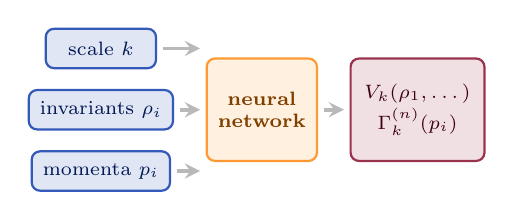
\begin{tikzpicture}[node distance=0.25cm and 0.4cm]
        \node[stage=Kleinblue, minimum width=1.4cm, minimum height=0.5cm, font=\scriptsize] (k)
          {scale $k$};
        \node[stage=Kleinblue, minimum width=1.4cm, minimum height=0.5cm, font=\scriptsize, below=of k] (f)
          {invariants $\rho_i$};
        \node[stage=Kleinblue, minimum width=1.4cm, minimum height=0.5cm, font=\scriptsize, below=of f] (p)
          {momenta $p_i$};
        \node[stage=orange, minimum width=1.4cm, minimum height=1.3cm, font=\scriptsize\bfseries, right=of f] (nn)
          {neural\\ network};
        \node[stage=burgundy, minimum width=1.7cm, minimum height=1.3cm, font=\scriptsize, right=of nn] (out)
          {$V_k(\rho_1,\dots)$\\[1pt] $\Gamma^{(n)}_k(p_i)$};
        \draw[tlarrow] (k.east) -- (nn.west|-k.east);
        \draw[tlarrow] (f.east) -- (nn.west);
        \draw[tlarrow] (p.east) -- (nn.west|-p.east);
        \draw[tlarrow] (nn) -- (out);
      \end{tikzpicture}\\[0.2em]
      \makebox[\linewidth]{\scriptsize universal approximators, strong representation power}\\[0.8em]
      \makebox[\linewidth][l]{physics-informed RG: \alert{Friederike's talk}}}
    \end{column}
  \end{columns}
  \refs{%
    \rtag{Physics-driven learning:} Aarts, Fukushima, Hatsuda, Ipp, Shi, Wang, Zhou, Nat.\ Rev.\ Phys.\ 7, 154 (2025).\quad
    \rtag{Vertex expansion in QCD:} Mitter, Pawlowski, Strodthoff, PRD 91, 054035 (2015); Fu, Huang, Pawlowski, Tan, Zhou, PRD 112, 054047 (2025).\quad
    \rtag{Operator learning:} DeepONet, Lu et al., Nat.\ Mach.\ Intell.\ 3, 218 (2021); FNO, Li et al., arXiv:2010.08895.\quad
    \rtag{Physics-informed kernels:} Ihssen, Pawlowski, Ann.\ Phys.\ 481, 170177 (2025); arXiv:2507.13011; Ihssen, Kapust, Pawlowski, arXiv:2510.26678; arXiv:2603.03159.}
\end{frame}

% ---------------------------------------------------------------- 1
\begin{frame}{The flow is stiff}
  \begin{columns}[T,onlytextwidth]
    \begin{column}{0.50\textwidth}
      \small
      \kb{$O(N)$ model, LPA (Model A)}
      \begin{equation*}
        \partial_t V_k=\mathscr{C}Tk^d\Big[
          \frac{1}{1+\bar m_{\sigma,k}^2}
          +\frac{N-1}{1+\bar m_{\pi,k}^2}\Big]
      \end{equation*}
      \vspace{-0.4em}
      \begin{equation*}
        \bar m_{\sigma,k}^2=\frac{V_k^{\prime}+2\rho V_k^{\prime\prime}}{k^2},\qquad
        \bar m_{\pi,k}^2=\frac{V_k^{\prime}}{k^2}
      \end{equation*}
      \vspace{-0.8em}

      \kb{Convexity restoration}

      $1+\bar m^2_{\sigma/\pi}\ge0$ at all $k$\\
      $\rho<\rho_0$: $V^{\,\prime}_k\to-k^2$, so $1+\bar m^2\to0^+$

      \vspace{0.3em}
      \kb{Stiffness in a narrow field window}

      propagators span \alert{$\bm{10^{-4}}$--$\bm{10^{2}}$},\\
      $\partial_t V^{\,\prime}$ spans $10^{2}$--$10^{7}$ ($k{=}20\MeV$)
    \end{column}
    \begin{column}{0.48\textwidth}
      \centering
      \includegraphics[width=\linewidth]{simga-pi-propagator}\\[0.2em]
      {\scriptsize $O(4)$, $T=100\MeV$, broken phase.}
    \end{column}
  \end{columns}
  \refs{%
    $\rho=\tfrac12\phi_a\phi_a$, $t=\ln(k/\Lambda)$, $\hat\rho=\rho/(\Lambda T_c)$.\quad
    \rtag{Model A:} Hohenberg, Halperin, RMP 49, 435 (1977).\quad
    \rtag{Flow equation from real-time fRG:} Tan, Chen, Fu, SciPost Phys.\ 12, 026 (2022); Chen, Tan, Fu, PRD 109, 094044 (2024).}
\end{frame}

% ---------------------------------------------------------------- 2
\begin{frame}{Learn only the finite-$N$ correction}
  \begin{columns}[T,onlytextwidth]
    \begin{column}{0.46\textwidth}
      \small
      \kb{Decomposition}
      \vspace{-0.3em}
      \begin{equation*}
        \hat V^{\,\prime}(t,\hat\rho)=\underbrace{\hat V^{\,\prime}_{\LN}(t,\hat\rho)}_{\text{analytic}}
        +\underbrace{\Delta\hat V^{\,\prime}_\theta(t,\hat\rho)}_{\text{network}}
      \end{equation*}
      \vspace{-0.4em}

      \kb{Large-$N$ flow}
      \vspace{-0.3em}
      \begin{equation*}
        \partial_t V_k=\mathscr{C}Tk^d\,\frac{N-1}{1+\bar m_{\pi,k}^2}
      \end{equation*}
      \vspace{-0.5em}

      solvable by characteristics:\\
      $V^{\,\prime}$ constant along them,\\
      $\rho_k$ in closed form (${}_2F_1$)

      \vspace{0.6em}
      \kb{Why it helps}\\
      large $N$ restores convexity;\\
      the rest is \alert{smooth and localized}
    \end{column}
    \begin{column}{0.54\textwidth}
      {\raggedright\hspace*{0.09\linewidth}\includegraphics[width=\linewidth]{T=100_deltaV}\par}
      \centering
      \vspace{0.1em}
      {\scriptsize Learned $\Delta\hat V^{\,\prime}_k(\hat\rho)$, $O(4)$, $T=100\MeV$.\\
      Zero at $k{=}\Lambda$, largest at $k\sim0.2$--$0.6\GeV$.}

      \vspace{1.2em}
      \small\raggedright
      \kb{Initial and boundary conditions}\\[0.2em]
      $\Delta\hat V^{\,\prime}_\theta(0,\hat\rho)=0$\\
      $\Delta\hat V^{\,\prime}_\theta(t,0),\ \Delta\hat V^{\,\prime}_\theta(t,\hat\rho_{\max})$: \alert{not specified}
    \end{column}
  \end{columns}
\end{frame}

% ---------------------------------------------------------------- 3
\begin{frame}{Solving the flow equation as an optimization problem}
  \relax % keep beamer from reading the next brace group as a subtitle
  {\centering
    \includegraphics[width=0.55\textwidth]{NN_architecture_LargeN}\\[-0.1em]
    {\scriptsize inputs $(t,\hat\rho)$ $\to$ simple nonlinear layers $\to$ output $\Delta\hat V^{\,\prime}_\theta$}\par}
  \vspace{0.4em}
  \small
  \kb{1.\ Residual}\quad insert $\hat V^{\,\prime}_{\LN}+\Delta\hat V^{\,\prime}_\theta$ into the flow equation on the grid:\\
  \hspace*{1.5em}$\mathcal R_{ij}(\theta)=\partial_t\hat V^{\,\prime}_\theta-\mathcal F[\hat V^{\,\prime}_\theta,\hat V^{\,\prime\prime}_\theta,\hat V^{\,\prime\prime\prime}_\theta]\big|_{(\hat\rho_i,t_j)}$,
  zero for the exact solution

  \vspace{0.4em}
  \uncover<2->{%
  \kb{2.\ Solve $=$ minimize}\quad $L(\theta)=\tfrac{1}{N_{\rm grid}}\sum_{ij}|\mathcal R_{ij}(\theta)|^2$ over $\theta$\\
  \hspace*{1.5em}gradient descent; the equation is the \alert{only input}, no training data}

  \vspace{0.4em}
  \uncover<3->{%
  \kb{Built in}\quad initial condition (output $\propto t$); no field boundary condition}
  \refs{%
    Details: 3-point finite differences on a $201\times501$ grid, $3$--$4\times$ less memory than autodiff; Adam; float32.\quad
    \rtag{PINN:} Raissi, Perdikaris, Karniadakis, JCP 378, 686 (2019); Karniadakis et al., Nat.\ Rev.\ Phys.\ 3, 422 (2021).\quad
    \rtag{PINNs for fRG / FDE / DSE:} Yokota, PRB 109, 214205 (2024); Miyagawa, Yokota, NeurIPS 2024; Terin, SciPost Phys.\ Core 8, 054 (2025).\quad
    \rtag{FD derivatives in PINNs:} Chiu et al., CMAME 395, 114909 (2022).}
\end{frame}

% ---------------------------------------------------------------- 4
\begin{frame}{Training}
  \begin{columns}[T]
    \begin{column}{0.50\textwidth}
      \centering
      \includegraphics[width=0.86\linewidth]{T=10_loss}\\[0.1em]
      {\scriptsize From scratch, $T{=}10\MeV$, $4{\times}10^6$ epochs}
    \end{column}
    \begin{column}{0.50\textwidth}
      \centering
      \includegraphics[width=0.86\linewidth]{T=100-200_loss}\\[0.1em]
      {\scriptsize Transfer from $T{=}120\MeV$, $5{\times}10^5$ epochs}
    \end{column}
  \end{columns}
  \vspace{0.8em}
  \begin{columns}[T,onlytextwidth]
    \begin{column}{0.31\textwidth}
      \centering
      \kb{Optimizer}\\[0.3em]
      \small Adam, lr $5\times10^{-4}$\\
      float32, then float64
    \end{column}
    \begin{column}{0.31\textwidth}
      \centering
      \kb{Domain}\\[0.3em]
      \small $k\in[20\MeV,1\GeV]$\\
      $\hat\rho\in[0,0.15]$\\
      grid $201\times501$
    \end{column}
    \begin{column}{0.31\textwidth}
      \centering
      \kb{Convergence}\\[0.3em]
      \small \alert{staircase} descent,\\
      plateau at $\sim10^{-9}$
    \end{column}
  \end{columns}
  \refs{%
    Grid $2001\times501$ and float64 refinement for the $T=10\MeV$ run.\quad
    Denominators regularized by $\epsilon=10^{-13}$.\quad
    PyTorch, PhysicsNeMo, Lightning.}
\end{frame}

% ---------------------------------------------------------------- 5
\begin{frame}{Broken phase: $\hat V^{\,\prime}_k(\hat\rho)$ vs. LDG and finite differences}
  \begin{columns}[T,onlytextwidth]
    \begin{column}{0.49\textwidth}
      \centering
      \includegraphics[width=\linewidth]{T=100_sol_2}\\[0.1em]
      {\scriptsize $T=100\MeV$, $k=100,80,50,20\MeV$}
    \end{column}
    \begin{column}{0.49\textwidth}
      \centering
      \includegraphics[width=\linewidth]{T=10_sol_2}\\[0.1em]
      {\scriptsize $T=10\MeV$, deeply broken, same $k$}
    \end{column}
  \end{columns}
  \vspace{0.8em}
  \begin{columns}[T,onlytextwidth]
    \begin{column}{0.31\textwidth}
      \centering
      \kb{Benchmarks}\\[0.3em]
      \small LDG and FD-BDF
    \end{column}
    \begin{column}{0.31\textwidth}
      \centering
      \kb{Accuracy}\\[0.3em]
      \small absolute error \alert{$\bm{<4\times10^{-5}}$}\\
      at all $k$ and $\hat\rho$
    \end{column}
    \begin{column}{0.31\textwidth}
      \centering
      \kb{Stiff region}\\[0.3em]
      \small no oscillations at the\\ crossover $\hat\rho_0(k)$
    \end{column}
  \end{columns}
  \refs{%
    \rtag{LDG benchmark (DiFfRG):} Sattler, Pawlowski, arXiv:2412.13043.}
\end{frame}

% ---------------------------------------------------------------- 6
\begin{frame}{Observables across the phase transition}
  \begin{columns}[T,onlytextwidth]
    \begin{column}{0.50\textwidth}
      \centering
      \includegraphics[width=0.76\linewidth]{rho_0_lowT}\\[-0.15em]
      \includegraphics[width=0.76\linewidth]{rho_0_highT}\\[0.3em]
      \small
      \kb{Order parameter} $\hat V^{\,\prime}(\hat\rho_0)=0$\\
      $T<T_c$: $\hat\rho_0$ finite,\ \ $T\ge T_c$: $\hat\rho_0\to0$
    \end{column}
    \begin{column}{0.50\textwidth}
      \centering
      \includegraphics[width=0.76\linewidth]{msig2_lowT}\\[-0.15em]
      \includegraphics[width=0.76\linewidth]{msig2_highT}\\[0.3em]
      \small
      \kb{Curvature mass}\\
      $\hat m_\sigma^2=\hat V^{\,\prime}(\hat\rho_0)+2\hat\rho_0\hat V^{\,\prime\prime}(\hat\rho_0)$
    \end{column}
  \end{columns}
\end{frame}

% ---------------------------------------------------------------- 7
\begin{frame}{Same idea for the Wilson--Fisher fixed point}
  \begin{columns}[T,onlytextwidth]
    \begin{column}{0.54\textwidth}
      \small
      \kb{Fixed-point equation, $d=3$, LPA}
      {\footnotesize
      \begin{equation*}
        0=-3u+\bar\rho u^{\mkern1.5mu\prime}
        +\mathscr{C}\Big[\frac{1}{1+u^{\mkern1.5mu\prime}+2\bar\rho u^{\mkern1.5mu\prime\prime}}+\frac{N-1}{1+u^{\mkern1.5mu\prime}}\Big]
      \end{equation*}}
      \vspace{-0.6em}

      \kb{Shooting is delicate}

      fine tuning to isolate WF from\\
      Gaussian and multicritical branches

      \vspace{0.5em}
      \kb{Network}

      $u^{\mkern1.5mu\prime}=u^{\mkern1.5mu\prime}_{\LN}+\Delta u^{\mkern1.5mu\prime}_\theta$\\
      $u^{\mkern1.5mu\prime}_{\LN}$ in closed form (${}_2F_1$)\\
      4-layer MLP, ODE residual loss

      \alert{no shooting, no Gaussian collapse}
    \end{column}
    \begin{column}{0.44\textwidth}
      \centering
      \includegraphics[width=0.92\linewidth]{fixedpoint_N=1-4_all}\\[0.1em]
      \includegraphics[width=0.92\linewidth]{fixedpoint_N=1-4_small}
    \end{column}
  \end{columns}
  \refs{%
    \rtag{Shooting benchmark:} Tan, Huang, Chen, Fu, EPJC 84, 897 (2024).}
\end{frame}

% ---------------------------------------------------------------- 8
\begin{frame}{The large-$N$ limit is not essential}
  \begin{columns}[T,onlytextwidth]
    \begin{column}{0.52\textwidth}
      \small
      \kb{Baselines from the equation itself}\\
      large field: $u^{\mkern1.5mu\prime}_*\to A\bar\rho^2$, $A=3\gamma\simeq84$\\[0.3em]
      {\centering $u^{\mkern1.5mu\prime}=A\bar\rho^2+\Delta u^{\mkern1.5mu\prime}_\theta$\par}

      \vspace{0.3em}
      \kb{Composite ansatz} ($O(1)$, $d=3$)
      \vspace{-0.4em}
      {\footnotesize
      \begin{equation*}
        \begin{aligned}
          u^{\mkern1.5mu\prime}_{\rm base}&=u^{\mkern1.5mu\prime}_{\rm poly}\,[1-w]+A\bar\rho^2\,w\\
          w&=\tfrac12\big\{1+\tanh\big[(\bar\rho-0.1)/0.02\big]\big\}
        \end{aligned}
      \end{equation*}}
      \vspace{-0.6em}

      $u^{\mkern1.5mu\prime}_{\rm poly}$: 10th-order Taylor series\\[0.3em]
      {\centering $u^{\mkern1.5mu\prime}=u^{\mkern1.5mu\prime}_{\rm base}+\Delta u^{\mkern1.5mu\prime}_\theta$\par}

      \vspace{0.3em}
      \uncover<2->{%
      \kb{Mistuned amplitude} $A/2$ or $2A$\\
      coarse grid: a spurious solution\\
      fine grid: \alert{WF recovered}, $A$ to $0.005\%$}
    \end{column}
    \begin{column}{0.46\textwidth}
      \centering
      \includegraphics[width=0.88\linewidth]{baseline_error}\\[0.3em]
      \uncover<2->{\includegraphics[width=0.88\linewidth]{baseline_finegrid_small}}
    \end{column}
  \end{columns}
  \refs{%
    \rtag{Large-field asymptotics, $A=3\gamma$:} Tan, Huang, Chen, Fu, EPJC 84, 897 (2024).}
\end{frame}

% ---------------------------------------------------------------- 10
\begin{frame}[c]{Summary}
  \relax % keep beamer from reading the next brace group as a subtitle
  {\centering\large Flow equation in the loss $\longrightarrow$ $V_k(\rho)$ as a neural network\par}
  \vspace{0.6em}
  \begin{columns}[T,onlytextwidth]
    \begin{column}{0.33\textwidth}
      \centering
      {\small Finite-$T$ $O(4)$ flows}\\[0.4em]
      {\alert{\large all three regimes}}\\[0.3em]
      {\footnotesize symmetric, broken, critical\\ error $<4\times10^{-5}$}
    \end{column}
    \begin{column}{0.33\textwidth}
      \centering
      {\small Key ingredient}\\[0.4em]
      {\alert{\large $\hat V^{\,\prime}=\hat V^{\,\prime}_{\LN}+\Delta\hat V^{\,\prime}_\theta$}}\\[0.3em]
      {\footnotesize stiffness absorbed\\ analytically}
    \end{column}
    \begin{column}{0.33\textwidth}
      \centering
      {\small Wilson--Fisher, $N\le4$}\\[0.4em]
      {\alert{\large no shooting}}\\[0.3em]
      {\footnotesize any baseline with the\\ right asymptotics}
    \end{column}
  \end{columns}
  \vspace{0.8em}
  {\centering\small
    Outlook: multi-field potentials, vertex expansion,\\ operator learning, links to physics-informed kernels\par}
  \vspace{0.6em}
  {\centering
    {\large Thank you!}\par}
\end{frame}

\end{document}
